\section{实验要求与实验目的}

\subsection{实验要求}
本实验围绕 AT89C51 单片机完成十字路口交通灯控制系统设计，要求如下：
\begin{enumerate}
  \item 使用 P1 口驱动东西、南北两个方向的红、黄、绿 LED 信号灯。
  \item 按交通放行顺序实现绿灯通行、绿灯闪烁提示、黄灯过渡和红灯等待。
  \item 使用 INT0 外部中断接入应急按钮，触发后进入全红状态，延时后恢复原交通状态。
  \item 在 Proteus 中完成电源、复位、晶振、灯组控制和外部中断电路连接，并完成仿真调试。
\end{enumerate}

\subsection{实验目的}
\begin{enumerate}
  \item 掌握 AT89C51 并行 I/O 口驱动多路 LED 负载的方法。
  \item 理解交通灯有限状态机的设计思路和状态切换关系。
  \item 学习 8051 外部中断 INT0 的初始化、入口设置、现场保护和中断返回。
  \item 提高 Proteus 仿真环境下软硬件联合调试能力。
\end{enumerate}

\subsection{总体设计思路}
系统以 P1 口输出六路交通灯控制信号，以 P3.2 作为 INT0 应急输入。正常运行时，程序按照“南北绿灯通行、南北黄灯过渡、东西绿灯通行、东西黄灯过渡”的顺序循环；当 INT0 按键触发时，程序保存当前 P1 状态，临时切换到东西、南北全红状态，延时结束后恢复中断前的灯态。

\section{Proteus 原理图与硬件电路说明}

\subsection{完整原理图}
\begin{figure}[H]
  \centering
  
\includegraphics[width=0.95\textwidth]{images/ProteusSchematic.PNG}
  \caption{实验三交通灯 Proteus 完整原理图}
\end{figure}

\subsection{分电路截图}
\begin{figure}[H]
  \centering
  
\includegraphics[width=0.72\textwidth]{images/power.PNG}
  \caption{单片机供电电路}
\end{figure}

\begin{figure}[H]
  \centering
  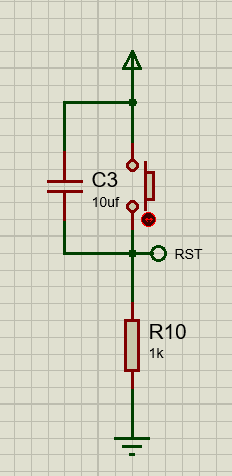
\includegraphics[width=0.58\textwidth]{images/rst.PNG}
  \caption{复位电路}
\end{figure}

\begin{figure}[H]
  \centering
  
\includegraphics[width=0.78\textwidth]{images/led_control.PNG}
  \caption{交通灯 LED 控制电路}
\end{figure}

\begin{figure}[H]
  \centering
  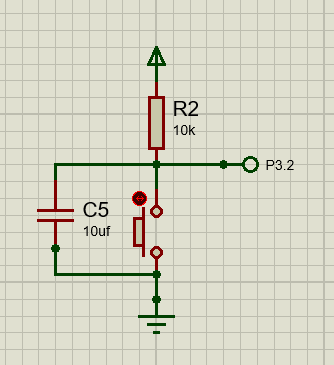
\includegraphics[width=0.58\textwidth]{images/INT.PNG}
  \caption{INT0 应急按键输入电路}
\end{figure}

\subsection{P1 口灯位分配}
\begin{table}[H]
  \centering
  \caption{P1 口交通灯控制位定义}
  \renewcommand{\arraystretch}{1.35}
  \begin{tabular}{clcl}
    \toprule
    端口位 & 控制对象 & 点亮电平 & 说明 \\
    \midrule
    P1.0 & 东西红灯 & 高电平 & 东西方向禁止通行 \\
    P1.1 & 东西绿灯 & 高电平 & 东西方向允许通行 \\
    P1.2 & 东西黄灯 & 高电平 & 东西方向通行结束提示 \\
    P1.3 & 南北红灯 & 高电平 & 南北方向禁止通行 \\
    P1.4 & 南北绿灯 & 高电平 & 南北方向允许通行 \\
    P1.5 & 南北黄灯 & 高电平 & 南北方向通行结束提示 \\
    \bottomrule
  \end{tabular}
\end{table}

\subsection{主要元件清单}
\begin{table}[H]
  \centering
  \caption{实验三主要元件与模型}
  \small
  \renewcommand{\arraystretch}{1.3}
  \begin{tabular}{cp{0.16\textwidth}p{0.22\textwidth}p{0.40\textwidth}}
    \toprule
    序号 & 元件名称 & 元件规格 & 功能说明 \\
    \midrule
    1 & 单片机 & AT89C51 & 主控制器，输出交通灯状态并响应 INT0 \\
    2 & 发光二极管 & LED-RED、LED-YELLOW、LED-GREEN & 模拟红、黄、绿交通信号灯 \\
    3 & 电阻 & RES & LED 限流保护 \\
    4 & 晶振 & CRYSTAL & 提供单片机运行时钟 \\
    5 & 电容 & CAP / CAP-ELEC & 晶振匹配、复位和滤波 \\
    6 & 按键 & BUTTON & 复位输入和 INT0 应急输入 \\
    7 & 电源端子 & POWER / GROUND & 提供 +5V 和公共地 \\
    \bottomrule
  \end{tabular}
\end{table}

\section{软件设计与程序流程}

\subsection{交通灯状态表}
\begin{table}[H]
  \centering
  \caption{正常循环与应急状态设计}
  \renewcommand{\arraystretch}{1.35}
  \begin{tabular}{clcl}
    \toprule
    状态 & P1 输出值 & 灯态说明 & 延时参数 \\
    \midrule
    初始/应急 & \texttt{09H} & 东西红灯，南北红灯 & R5=5 或 R5=10 \\
    S1 & \texttt{11H} & 东西红灯，南北绿灯 & R5=15 \\
    S1 闪烁间隔 & \texttt{01H} & 东西红灯，南北绿灯熄灭 & R5=2 \\
    S2 & \texttt{21H} & 东西红灯，南北黄灯 & R5=5 \\
    S3 & \texttt{0AH} & 南北红灯，东西绿灯 & R5=15 \\
    S3 闪烁间隔 & \texttt{08H} & 南北红灯，东西绿灯熄灭 & R5=2 \\
    S4 & \texttt{0CH} & 南北红灯，东西黄灯 & R5=5 \\
    \bottomrule
  \end{tabular}
\end{table}

\subsection{程序流程图}
\begin{figure}[H]
\centering
\begin{tikzpicture}[
  node distance=9mm and 14mm,
  proc/.style={rectangle,rounded corners,draw=themecolor,fill=blue!3,minimum width=5.8cm,minimum height=8mm,align=center},
  warn/.style={rectangle,rounded corners,draw=accentyellow,fill=yellow!8,minimum width=5.8cm,minimum height=8mm,align=center},
  io/.style={trapezium,trapezium left angle=75,trapezium right angle=105,draw=themecolor,fill=cyan!6,minimum width=5.8cm,minimum height=8mm,align=center},
  line/.style={-Latex,thick,draw=themecolor}
]
  \node[proc] (start) {程序开始，设置堆栈};
  \node[proc,below=of start] (intinit) {初始化 INT0：\texttt{SETB IT0 / EX0 / EA}};
  \node[io,below=of intinit] (allred) {输出全红：\texttt{MOV P1,\#09H}};
  \node[proc,below=of allred] (nsgreen) {南北绿，东西红};
  \node[proc,below=of nsgreen] (nsflash) {南北绿灯闪烁 3 次};
  \node[warn,below=of nsflash] (nsyellow) {南北黄，东西红};
  \node[proc,below=of nsyellow] (ewgreen) {东西绿，南北红};
  \node[proc,below=of ewgreen] (ewflash) {东西绿灯闪烁 3 次};
  \node[warn,below=of ewflash] (ewyellow) {东西黄，南北红};

  \draw[line] (start) -- (intinit);
  \draw[line] (intinit) -- (allred);
  \draw[line] (allred) -- (nsgreen);
  \draw[line] (nsgreen) -- (nsflash);
  \draw[line] (nsflash) -- (nsyellow);
  \draw[line] (nsyellow) -- (ewgreen);
  \draw[line] (ewgreen) -- (ewflash);
  \draw[line] (ewflash) -- (ewyellow);
  \draw[line] (ewyellow.east) -| ++(1.5,0) |- (nsgreen.east);
\end{tikzpicture}
\caption{交通灯主程序流程图}
\end{figure}

\subsection{INT0 应急中断流程}
\begin{figure}[H]
\centering
\begin{tikzpicture}[
  node distance=9mm and 13mm,
  proc/.style={rectangle,rounded corners,draw=themecolor,fill=blue!3,minimum width=5.8cm,minimum height=8mm,align=center},
  redstate/.style={rectangle,rounded corners,draw=accentred,fill=red!6,minimum width=5.8cm,minimum height=8mm,align=center},
  line/.style={-Latex,thick,draw=themecolor}
]
  \node[proc] (irq) {INT0 下降沿触发};
  \node[proc,below=of irq] (save) {保存 ACC、R5、R6、R7};
  \node[proc,below=of save] (p1save) {读取并保存当前 P1 状态};
  \node[redstate,below=of p1save] (emg) {输出 \texttt{09H}，东西南北全红};
  \node[proc,below=of emg] (restore) {恢复中断前 P1 状态};
  \node[proc,below=of restore] (reti) {恢复寄存器并 \texttt{RETI}};

  \draw[line] (irq) -- (save);
  \draw[line] (save) -- (p1save);
  \draw[line] (p1save) -- (emg);
  \draw[line] (emg) -- (restore);
  \draw[line] (restore) -- (reti);
\end{tikzpicture}
\caption{INT0 应急中断处理流程图}
\end{figure}

\subsection{交通灯状态时序}
\begin{figure}[H]
\centering
\begin{tikzpicture}[
  x=0.85cm,y=0.72cm,
  axis/.style={draw=softline,thick},
  phase/.style={draw=themecolor,rounded corners=2pt,minimum height=0.52cm,align=center,font=\small},
  red/.style={phase,fill=red!12,draw=accentred},
  green/.style={phase,fill=green!12,draw=accentgreen},
  yellow/.style={phase,fill=yellow!18,draw=accentyellow}
]
  \node[anchor=east] at (0,3) {南北};
  \node[anchor=east] at (0,1.8) {东西};
  \node[green,minimum width=4.2cm] at (2.2,3) {绿};
  \node[yellow,minimum width=1.5cm] at (5.15,3) {黄};
  \node[red,minimum width=5.2cm] at (8.5,3) {红};
  \node[red,minimum width=5.7cm] at (2.95,1.8) {红};
  \node[green,minimum width=4.2cm] at (7.9,1.8) {绿};
  \node[yellow,minimum width=1.5cm] at (10.85,1.8) {黄};
  \draw[axis] (0,0.9) -- (11.6,0.9);
  \foreach \x/\t in {0/开始,4.4/南北黄,5.9/东西绿,10.1/东西黄,11.6/循环}
    \draw[axis] (\x,0.75) -- (\x,1.05) node[below=4pt,font=\small] {\t};
\end{tikzpicture}
\caption{正常交通灯状态时序示意图}
\end{figure}

\subsection{完整实验代码}
\lstset{style=a51style}
\lstinputlisting[caption={03\_traffic\_light.A51 完整源码}]{code/03_traffic_light.A51}

\subsection{关键代码说明}
\begin{table}[H]
  \centering
  \caption{关键指令与功能说明}
  \renewcommand{\arraystretch}{1.35}
  \begin{tabular}{p{0.32\textwidth}p{0.62\textwidth}}
    \toprule
    指令或语句 & 功能说明 \\
    \midrule
    \texttt{ORG 0003H / LJMP INT0\_ISR} & 设置 INT0 外部中断入口，使应急按钮触发后进入中断服务程序。 \\
    \texttt{SETB IT0} & 配置 INT0 为下降沿触发，适合按键输入产生的触发信号。 \\
    \texttt{SETB EX0 / SETB EA} & 分别打开 INT0 中断允许位和总中断允许位。 \\
    \texttt{MOV P1,\#11H} & 输出东西红灯、南北绿灯，对应南北方向通行。 \\
    \texttt{MOV P1,\#21H} & 输出东西红灯、南北黄灯，对应南北方向由通行转为停止的过渡状态。 \\
    \texttt{MOV P1,\#0AH} & 输出南北红灯、东西绿灯，对应东西方向通行。 \\
    \texttt{MOV P1,\#09H} & 输出东西红灯、南北红灯，用于初始状态和应急全红状态。 \\
    \texttt{PUSH / POP / RETI} & 完成中断现场保护、现场恢复和中断返回。 \\
    \bottomrule
  \end{tabular}
\end{table}

\section{调试过程与实验结果}

\subsection{调试过程记录}
\begin{enumerate}
  \item 在 Proteus 中完成 AT89C51、供电、复位、晶振、交通灯 LED 和 INT0 应急按键连接。
  \item 将交通灯汇编程序加载到 AT89C51，检查复位入口和 INT0 中断入口地址是否正确。
  \item 启动仿真，观察初始状态是否为东西、南北全红。
  \item 连续观察正常循环，确认南北通行、南北黄灯、东西通行、东西黄灯顺序正确。
  \item 在不同灯态下按下 INT0 应急按键，检查是否立即进入全红状态，并在延时后恢复原灯态。
\end{enumerate}

\subsection{结果验证表}
\begin{table}[H]
  \centering
  \caption{交通灯仿真结果记录}
  \renewcommand{\arraystretch}{1.35}
  \begin{tabular}{clcc}
    \toprule
    序号 & 测试内容 & 预期现象 & 结果 \\
    \midrule
    1 & 上电复位 & 东西红灯、南北红灯点亮 & 符合 \\
    2 & 正常循环第一阶段 & 南北绿灯亮，东西红灯亮 & 符合 \\
    3 & 南北通行结束提示 & 南北绿灯闪烁后切换为南北黄灯 & 符合 \\
    4 & 正常循环第二阶段 & 东西绿灯亮，南北红灯亮 & 符合 \\
    5 & 东西通行结束提示 & 东西绿灯闪烁后切换为东西黄灯 & 符合 \\
    6 & INT0 应急按键 & 立即进入全红，延时后恢复中断前灯态 & 符合 \\
    \bottomrule
  \end{tabular}
\end{table}

\subsection{程序正确性分析}
程序采用固定状态表输出 P1 端口值，逻辑关系清晰：任意时刻两个方向不会同时出现绿灯，从而避免交通冲突。INT0 中断服务程序在进入时保存 ACC、R5、R6、R7，并额外保存 P1 当前值，确保应急全红结束后可以恢复原来的交通灯显示状态。

\section{问题分析与改进建议}
\begin{enumerate}
  \item 当前延时由软件循环完成，时间精度受晶振频率和指令周期影响；实际系统中可改用定时器中断获得更稳定的秒级计时。
  \item INT0 使用机械按键时可能产生抖动，硬件上可加入 RC 滤波，软件上可在中断入口增加短延时消抖。
  \item 交通灯状态目前采用顺序代码展开，若后续扩展倒计时数码管，可将状态、输出值和延时参数整理为表驱动结构。
\end{enumerate}

\section{实验结论}
本实验完成了基于 AT89C51 的交通灯控制系统设计与仿真。程序通过 P1 口输出东西、南北两个方向的红黄绿灯控制信号，实现了正常通行、绿灯闪烁、黄灯过渡和循环切换；同时利用 INT0 外部中断实现应急全红功能。仿真结果表明，硬件连接、端口输出和中断处理均满足实验要求。
